\chapter{Implementation and Experimental Results}
\label{sec:impl}

Julia is a multi-paradigm language created by \citeauthor{Julia} at the Massachusetts Institute of Technology~(MIT)~\cite{Julia}.
While development on the language began in~2009, its version~1.0 has been released in 2018.
This chapter first covers the general properties of the two Julia packages created during the work on this thesis.
Both of these packages have an automated test suite with a coverage of well over \SI{90}{\percent}.
Lastly, the packages are applied to the Rail benchmark problem~\cite{morwiki_steel}.

\section{DifferentialRiccatiEquations.jl}
\label{sec:impl:DRE}

% Don't mention the inconsistency in tspan!  I was inspired by Norman's code,
% which received tspan sorted, i.e. in forwards time, and internally reversed
% it before and after solving.  Not knowing what I was doing, I thought
% accepting tspan in backwards time was a clever idea.  Now this package has to
% be used with backwards tspan, while having the equations stated in forwards
% time.
%
% https://gitlab.mpi-magdeburg.mpg.de/jschulze/DifferentialRiccatiEquations.jl/-/issues/6#note_13652

This package is concerned with sequential \ac{DRE} solvers only.
The general user interface has been inspired by \code{DifferentialEquations.jl}~\cite{DifferentialEquations},
and looks like this:
\begin{lstlisting}[
  caption={[User interface of \code{DifferentialRiccatiEquations.jl}]},
]
prob = GDREProblem(E, A, B, C, X0, tspan)
alg = Ros1()
sol = solve(prob, alg; dt=dt)
\end{lstlisting}
Besides \julia{Ros1()} and \julia{Ros2()},
which correspond to the algorithms described in \autoref{sec:ros},
there also is a \julia{Ros4()} solver.
It is based on \citeauthor{Lang2017}~\cite[Appendix~A]{Lang2017} and only supports the dense case.
The \julia{GDREProblem} type is parametrized on the type of the initial value \julia{X0},
by which the proper \ac{ALE} solver is selected via runtime dispatch on \julia{solve()}.
Dense initial values are represented by the built-in \julia{Matrix} type,\footnote{%
  \url{https://docs.julialang.org/en/v1.6/stdlib/LinearAlgebra/}}
and lead to a direct \ac{ALE} solver from \code{MatrixEquations.jl}~\cite{MatrixEquations}.
Initial values in \ac{LRSIF} are represented by the new \julia{\LDLt} type,
and lead to the iterative \ac{ADI} solver described in \autoref{sec:ADI}.

\paragraph{Representation of Low-Rank Matrices}

Suppose $X = LDL^\T$ and \julia{X = \LDLt(L, D)} are mathematical and Julia representations of the same objects,
$L\in\R^{n\times r}$, $D\in\R^{r\times r}$.
Then, the internal representation of~\julia{X} consists of lists~\julia{[L]} and~\julia{[D]},
such that updates may be performed lazily by merely collecting all the summands,
\cf \autoref{sec:lowrank}.
Compression of~\julia{X} is performed once these lists contain 10 elements or more,
or if the equivalent inner dimension is too large, $r \geq \onehalf n$.
This causes a compression every 10 iterations of the \ac{ADI} or earlier.
This is not configurable yet,
\cf~\autoref{lst:impl:LDLt}.
Note that line~\ref{line:impl:LDLt:compression_due} mainly guards the situation
when a user accesses $L$ and $D$ (via iteration: \mbox{\julia{L, D = X}}),
compression is not performed twice.
All internal usages guarantee the assumption in the comment above line~\ref{line:impl:LDLt:compression_due}.

\begin{lstlisting}[
  float=tp,
  caption={%
    [{Definition of \julia{\LDLt} and \julia{(+)}}]
    Definition of \julia{\LDLt} and addition \julia{(+)} of \ac{LRSIF} objects.
    The compression, \julia{compress!()}, is described in \autoref{alg:lowrank:compression}.
  },
  label={lst:impl:LDLt},
  escapechar=\%,
]
struct %\LDLt%{TL,TD}
    Ls::Vector{TL}
    Ds::Vector{TD}
end

function Base.:(+)(Xs::%\LDLt%{TL,TD}...) where {TL,TD}
    Ls = TL[]
    Ds = TD[]
    for X in Xs
        append!(Ls, X.Ls)
        append!(Ds, X.Ds)
    end
    X = %\LDLt%{TL,TD}(Ls, Ds)
    maybe_compress!(X)
end

function compression_due(X::%\LDLt%)
    # If there is only one component, it has likely already been compressed:
    length(X.Ls) == 1 && return false%\label{line:impl:LDLt:compression_due}%
    # Compression is due every couple of modifications:
    length(X.Ls) >= 10 && return true
    # Compression is due if rank is too large:
    n = size(X, 1)
    r = rank(X)
    return r >= 0.5n
end

function maybe_compress!(X::%\LDLt%)
    compression_due(X) || return X
    compress!(X)
end
\end{lstlisting}

\paragraph{Representation of Shifted Matrices}

Recall that the Rosenbrock methods yield \acp{ALE},
whose system matrices are sparse matrices shifted by a low-rank matrix,
\cf $\tilde A_n$ in \autoref{alg:ros1:smw} of \autoref{alg:ros1} and $\hat A_n$ in \autoref{alg:ros2:smw} of \autoref{alg:ros2}.
Within the \ac{ADI}, these matrices are updated by another sparse matrix,
\cf $A^+_k$ in \autoref{alg:ADI:smw} of \autoref{alg:ADI}.
Overall, taking \Ros{1} as an example,
the system to be solved with is
\begin{equation}
  A_k^+ =
  \big(\big( A_n - \tfrac{1}{2\tau} E \big)^\T + \alpha_k E \big) - K_n^\T B^\T
  .
\end{equation}
This structure, however, is completely hidden from the \ac{ADI} code via
\begin{lstlisting}[
  caption={[Abstraction of shifted linear system between Rosenbrock method and ADI]},
  %caption={Representation of shifted linear systems},
  escapechar=\%,
]
%\~A% = LowRankUpdate(A - E/(2%$\tau$%), -1, B, K)
R = %\LDLt%(G, S)
lyap = GALEProblem(E, %\~A%, R)
solve(lyap, ADI())
\end{lstlisting}
Thereby, the \ac{ADI} transposes $\tilde A$ via \julia{adjoint()},
%\footnote{%
%  In Julia, \julia{A'} is syntactic sugar for \julia{adjoint(A)},
%  \cf \url{https://docs.julialang.org/en/v1.6/manual/functions/\#Operators-With-Special-Names}
%}
and adds the sparse $\alpha_k E$ via \julia{(+)} without losing the \julia{LowRankUpdate} structure.
Its main feature, however, is solving the corresponding linear system via the backslash operator~\julia{(\textbackslash)}
using the Sherman-Morrison-Woodbury formula,
\cf \autoref{sec:basics:smw}.
See \autoref{lst:impl:LowRankUpdate} for the basic definition of \julia{LowRankUpdate} and the aforementioned functions.

\def\mi{\textsuperscript{-1}}
\def\ma{\protect\makebox[\widthof{a}]{$\alpha$}}
\begin{lstlisting}[
  float=tp,
  caption={%
    [{Definition of \julia{LowRankUpdate} as well as \julia{(+)} and \julia{(\textbackslash)}}]
    Definition of \julia{LowRankUpdate},
    a lazy representation of the shifted linear system $A + \alpha^{-1} UV$,
    as well as addition \julia{(+)} of a sparse matrix,
    and left-division \julia{(\textbackslash)}
    using the Sherman-Morrison-Woodbury formula,
    \cf \autoref{sec:basics:smw}.
  },
  label={lst:impl:LowRankUpdate},
  escapechar=\%,
]
struct LowRankUpdate{TA,T,TU,TV}
    A::TA
    %\ma%::T
    U::TU
    V::TV
end

function Base.adjoint(AUV::LowRankUpdate)
    A, %\ma%, U, V = AUV
    LowRankUpdate(A', %\ma%', V', U')
end

function Base.:(+)(AUV::LowRankUpdate, E::AbstractMatrix)
    @assert issparse(E)
    A, %\ma%, U, V = AUV
    LowRankUpdate(A+E, %\ma%, U, V)
end

function Base.:(\)(AUV::LowRankUpdate, B::AbstractVecOrMat)
    A, %\ma%, U, V = AUV

    FA = factorize(A)
    A%\mi%B = FA \ B
    A%\mi%U = FA \ U

    S = %\ma% * I + V * A%\mi%U
    S%\mi%VA%\mi%B = S \ (V * A%\mi%B)

    X = A%\mi%B - A%\mi%U * S%\mi%VA%\mi%B
    return X
end
\end{lstlisting}

% Above listing used to contain `_factorize`, which is a custom implementation.
% It's only purpose was to ensure that if the factorization is a `Diagonal`,
% its diagonal is a dense vector. In some of my dummy experiments, this was
% faster to solve with. However, A and E are basically never diagonal, so this
% function exists for "historical reasons" (TM) only.


\section{ParaReal.jl}

This section describes the general properties of the \julia{ParaReal.jl} package.
It has been designed with the following requirements in mind:
\begin{enumerate}
  \item\label{item:impl:goal:schedule}
    Schedule each stage on a separate process.

    This is a sensible default for the application at hand,
    which is memory bound for typical problem sizes.
    Yet, the scheduling strategy should be modifiable/extendable.
  \item\label{item:impl:goal:variablesize}
    Allow the data transferred be variable in size.

    This is necessary to transmit \ac{LRSIF} of varying rank and, therefore, storage size depending on $n$ (and $k$).
  \item\label{item:impl:goal:notransfer}
    Do not transfer the final solution data back to the calling/managing process.

    For fine resolutions, the storage requirements are immense.
    The overall solution might not fit in memory of a single compute node.
    Therefore, it has to be possible that each stage $n$ saves its local (fine) solution along $[t_{n-1},t_n]$ directly to disk,
    without sending it to the calling process first.
\end{enumerate}
On top of that:
\begin{enumerate}[resume]
  \item\label{item:impl:goal:modularity}
    The parareal implementation has to be modular,
    \ie easy to use/adapt for other problems than \ac{LRSIF} formulations of \ac{DRE}.
\end{enumerate}

Requirement \ref{item:impl:goal:schedule} is achieved by the abstract type \julia{Schedule},
whose sole subtype (for now) is \julia{ProcessesSchedule}.
It takes a list of $N$ worker/process ids, each of which will execute one stage.
Future strategies may be implemented by defining new subtype of \julia{Schedule}, \eg
\julia{ThreadsSchedule} using threads on a single process,
\julia{HybridSchedule} which uses both threads and processes, and
\julia{DaggerSchedule} which uses the abstractions provided by \julia{Dagger.jl}.\footnote{\url{https://github.com/JuliaParallel/Dagger.jl}}

Requirement \ref{item:impl:goal:variablesize} is trivial to fulfill using Julia's \julia{RemoteChannel} data type.
Requirement \ref{item:impl:goal:modularity} imposes a non-specific naming scheme for
user interface functions and the name of the unknown,
as to not clash with the standard nomenclatures of other disciplines.\footnote{%
  For example,
  many parareal papers use $U$ to name the unknown,
  many matrix \ac{ODE} papers use $X$,
  and the widely-used \julia{DifferentialEquations.jl} package~\cite{DifferentialEquations} uses $u$.
}
The next section will describe the user interface of the \julia{ParaReal.jl} package,
and how to cope with problem~\ref{item:impl:goal:notransfer}.

\subsection{User Interface}

In applications one is usually interested in a high temporal resolution,
while the parareal method is only used to obtain \enquote{fast} convergence.
Therefore, the \julia{ParaReal.jl} package distinguishes between a local solution along $[t_{n-1}, t_n]$ and the final value of which,
\begin{align*}
  F(U_{n-1}^k) &= \julia{value(fsolve(prob))} \\
  G(U_{n-1}^k) &= \julia{value(csolve(prob))}
\end{align*}
where \julia{prob} is an instance of the global \ac{IVP}~\eqref{eq:IVP}
restricted to the local time slice~$[t_{n-1}, t_n]$ and initial value~$U_{n-1}^k$.
The actual solver functions \julia{csolve} (\enquote{coarse}) and \julia{fsolve} (\enquote{fine})
are provided as arguments to \julia{ParaReal.Algorithm()}.
In order to support custom \ac{IVP} types,
a user has to defined methods for \julia{initial\_value()} to extract the global initial value $U_0$,
and \julia{remake\_prob()} to adjust the global problem for the local time slice and initial value.
For more details, refer to the documentation of the respective functions available from within Julia.

In order to support new solution types,
a custom implementation of the parareal update formula~\eqref{eq:pr:method} may be needed.
This can be specified as an optional third argument to \julia{ParaReal.Algorithm}.
The default is \julia{ParaReal.default\_update!()},
whose implementation is given in~\autoref{lst:impl:default_update!}.
Adding methods to \julia{default\_update!()} is not recommended.
Any custom implementation of the parareal update formula must follow the interface of \julia{default\_update!()}.

\def\sk{\textsuperscript{k}}
\def\skmi{\textsuperscript{k-1}}
\lstinputlisting[%
  float=t,
  label={lst:impl:default_update!},
  caption={Default implementations of the parareal update formula},
  escapechar=\%,
  breaklines=true,
]{code/default_update.jl}
% The form a+b+(-c) is for historical reasons. The LDLt data structure used to eagerly concatenate the
% matrices instead of collecting them lazily, as it does now. Back then, using a ternary plus meant
% fewer allocations (then: 2 allocs for L and 2 allocs for D, now: 0 allocs for L and 1 alloc for D)
% before compression.

The remainder of this section is devoted to a complete example of a user-defined problem type ($N=3$, $K=2$).
The problem type will be a mere placeholder that forwards its initial value,
while the solver functions will count the applications of $F$ and $G$ a particular solution is composed of.
Start by launching some worker processes and loading the necessary packages:
\lstinputlisting[%
  caption={User-defined problem type for \julia{ParaReal.jl}},
  label={lst:impl:parareal_counting},
  lastline=4,
]{code/parareal_counting.jl}
Next, define the problem type and ensure that definition is available on all processes.
The only requirement to the problem type is to have a \julia{tspan} field.\footnote{%
  Alternatively, it must support \julia{getproperty(prob, :tspan)}.
}
In the context of \ac{ODE}, this should not clash with any other notation.
\addtocounter{lstnumber}{1} %FIXME
\lstinputlisting[nolol, firstnumber=last, linerange=problem-end]{code/parareal_counting.jl}
The solution type will hold counters of the applications of $F$ and $G$:
\lstinputlisting[nolol, firstnumber=last, linerange=solution-end]{code/parareal_counting.jl}
Define the solver functions and problem instance and execute the parareal pipeline.
The solver functions are defined as closures,
such that they can be serialized and transferred to the worker processes.
Note that this code is only executed on the managing process:
\lstinputlisting[nolol, firstnumber=last, linerange=solve-end]{code/parareal_counting.jl}
Lastly, extracting the final values $U_1^1$, $U_2^2$, and $U_3^2$ via
\lstinputlisting[nolol, firstnumber=last, linerange=result-end]{code/parareal_counting.jl}
yields:
\begin{align*}
  &\julia{Counters(1,0)}, \text{ since} &
  U_1^1 &= F(U_0) \\
  &\julia{Counters(2,0)}, \text{ since} &
  U_2^2 &= F(F(U_0)) \\
  &\julia{Counters(3+2+2,2+4+4)}, \text{ since} &
  U_3^2 &= G(F(F(U_0))) + F(U_2^1) - G(U_2^1) \\
  && U_2^1 &= G(F(U_0)) + F(G(U_0)) - G(G(U_0))
\end{align*}

The full trajectory of the fine solver may be extracted using \julia{ParaReal.solution()}.
However, solution and value are identical in the example above,
\cf line~\ref{line:impl:parareal_counting:value}.
\autoref{lst:impl:store} shows the recommended pattern of
storing the fine solutions directly from the worker processes
via \julia{ParaReal.fetch\_from\_owner()}.

\lstinputlisting[%
  float=tpb, % TODO: ensure this doesn't disrupt the inline code snippets
  caption={%
    [Store fine parareal solutions directly from the worker processes]
    Store fine parareal solutions directly from the worker processes.
    This works well as a blueprint for \julia{DrWatson.\_wsave(dir, sol)} \cite{DrWatson}.
  },
  label={lst:impl:store},
]{code/parareal_store.jl}

\subsection{JIT Compilation and Warm-Up}

Julia is a \ac{JIT} compiled language~\cite{Julia},
which means that code is compiled just before it is first executed,
unless it has already been compiled.
Therefore, unless the code has been compiled \ac{AOT},
only the second execution of code is fast.
This effect is called \emph{warm-up}.
As mentioned in~\autoref{sec:pr}, computing the coarse solutions
$G(U_n^*)$ is essentially a sequential operation over all $n$.
The computations of $F(U^*_n)$ can only be parallelized after such a global coarse solve.
Therefore, it is critical that the individual coarse solutions are available as fast as possible.

In order to describe the runtime of the present parareal implementation,
let $t_F$, $t_G$ denote the runtime of $F$ and $G$, respectively.
Let $N$ be the number of stages $1 \leq n \leq N$,
and $K$ be the number of refinements $0 \leq k \leq K$.
Let $\trampup$ be the overhead imposed on each computing the first coarse solution $G(U_n^0)$,
and $\twarmup$ be a general global overhead.
Further, we make the following assumptions:
\begin{enumerate}
  \item
    $t_F$ and $t_G$ are constant, \ie do not depend on $n, k$.
  \item
    \label{item:impl:assumption:tU}
    The time to compute the actual value $U_n^k$ is negligible,
    \cf~\autoref{lst:impl:default_update!}.
  \item
    The overhead to check for convergence is negligible.
  \item
    Communication time is negligible.
  \item
    All stages $n$ compute $K$ refinements, \ie $k_n = K \enspace\forall n$.
\end{enumerate}
The runtime may then be estimated using
\begin{equation}
\label{eq:impl:tpar}
  \hattpar
  = \twarmup
  + \underbrace{
    \strut
    N \cdot (\trampup + t_G)
  }_{\substack{
    \text{stages $1\leq n\leq N$}\\
    \text{refinement $k=0$}
  }}
  + \underbrace{
    \strut
    K \cdot (t_F + t_G)
  }_{\substack{
    \vphantom{\text{stage}}
    n = N \\
    1 \leq k \leq K
  }}
  + t_F
\end{equation}
where the final $t_F$ is to compute the best fine solution available.
These assumptions are compatible to the generic timeline \autoref{fig:timeline:generic}.
As will be described later,
\begin{equation}
  \twarmup + \trampup
  = t_{\JIT(G)} + t_\text{other}
\end{equation}
\ie the goal is to offset/reduce the ramp-up delay $\trampup$
at the cost of a one-time overhead $\twarmup$.
$t_{\JIT(G)}$ denotes the compile time of $G$.
Refer to \autoref{tab:impl:warmup} for the measurements corresponding to \autoref{fig:impl:warmup}.

\begin{figure}[p]
  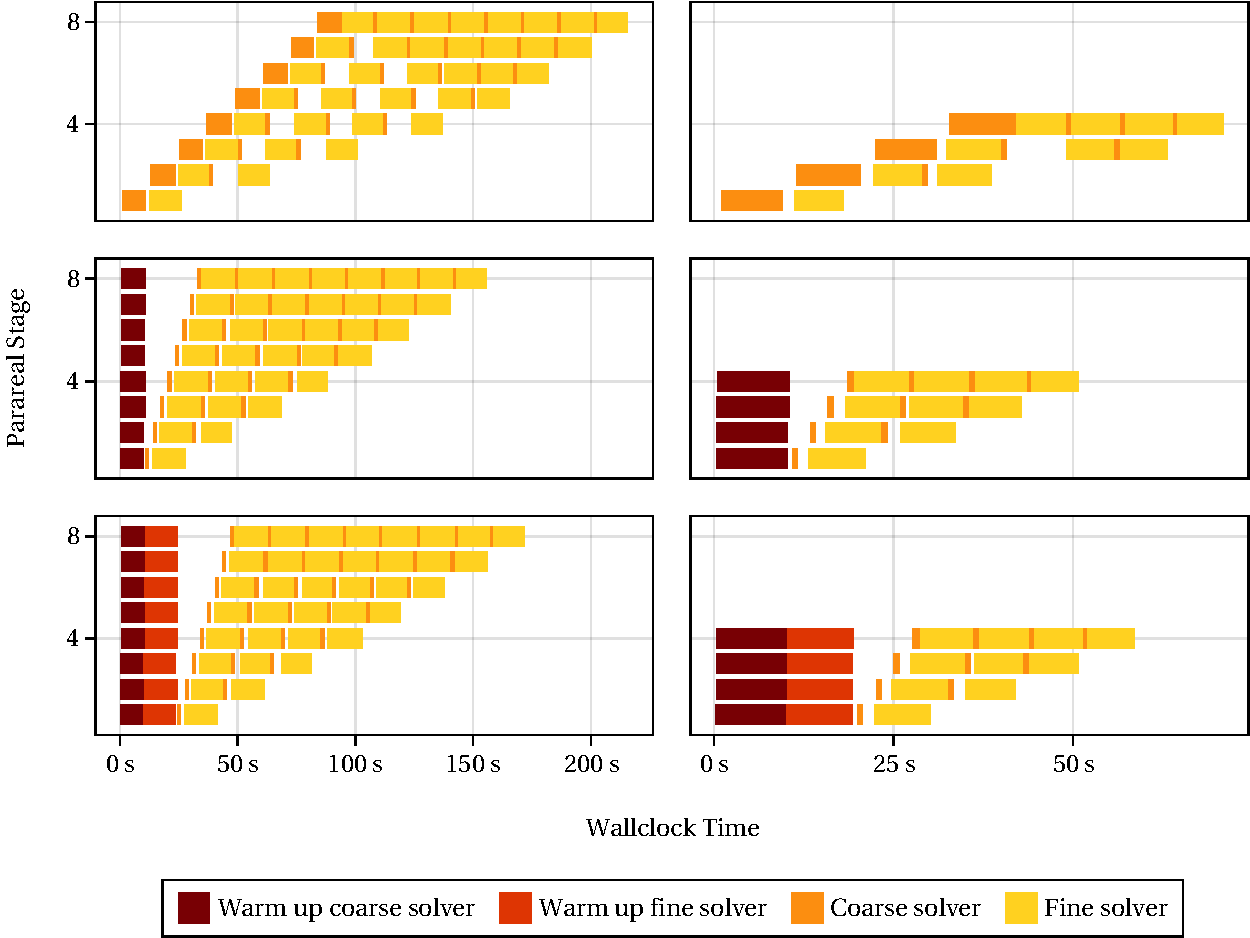
\includegraphics[width=\textwidth]{figures/fig_impl_warmup2.pdf}
  \caption[Timeline diagrams comparing the effect of JIT compiler warm-up]{%
    Timeline diagrams comparing the effect of \acs{JIT} compiler warm-up.
    Left: $N=8$ processes running on two compute nodes,
    right: $N=4$ processes running on a laptop.
    Top: no warm-up,
    middle: warming up coarse solver $G$ (\julia{csolve}),
    bottom: warming up coarse and fine solver $F$ (\julia{fsolve}).
  }
  \label{fig:impl:warmup}
\end{figure}

\begin{table}[p]
  \centering
  \begin{tabular}{lccccccc}
    \toprule
    warm-up & $N$ & $\twarmup$ & $\trampup$ & $t_G$ & $t_F$ & $\tpar$ & $\hattpar$ \\
    \midrule
    none  & 8 \\
    $G$   & 8 \\
    $G,F$ & 8 \\
    \midrule
    none  & 4 \\
    $G$   & 4 \\
    $G,F$ & 4 \\
    \bottomrule
  \end{tabular}
  \caption[Measurements corresponding to \autoref*{fig:impl:warmup}]{%
    Measurements corresponding to \autoref*{fig:impl:warmup}
    based on~\eqref{eq:impl:tpar}.
    The actual runtime is denoted by $\tpar$.
    $t_F$ and $t_G$ are estimated as the median,
    $\twarmup$ as the maximum of their respective runtimes.
    $\trampup$ is taken as the mean delay between adjacent $G(U_n^0)$.
    All timings are in seconds.
  }
  \label{tab:impl:warmup}
\end{table}

\paragraph{Sequential \ac{JIT} compilation}

Without any precautions,
\begin{equation*}
  \twarmup = 0,
\end{equation*}
\ac{JIT} compilation of $G$ happens sequentially,
as computing $G(U_n^k)$ is essentially sequential over $n$.
This effect is especially severe if the executors of different parareal iterations $(n,k)$ do not share the results of code compilation.
These executors may be processes, threads~(pthreads), or tasks~(green threads).
For the present implementation,
there is a one-to-one mapping between processes and stages $n$,
which means the compilation happens exactly once per stage $n$ and is reused between refinements $k$.\footnote{%
  As of the writing of this thesis, Julia does not reuse code compiled between processes.
}
This is visible in the first row of \autoref{fig:impl:warmup}
by the first occurrences of $G$ for each stage $n$,
which marks the computation of $G(U_n^0)$,
whose execution time includes compilation time.
Therefore, the first occurrences of $G$ take substantially longer than the subsequent ones.
The computation of the parareal update has a negligible duration,
and is therefore not shown in the timeline plot,
\cf assumption~\ref{item:impl:assumption:tU}.

\paragraph{Parallel \acs{AOT} compilation}

Since \julia{ParaReal.jl} is independent of $F$ and $G$ as well as the actual data type of the underlying \ac{IVP},
full \ac{AOT} compilation is difficult, and has to be done by users of the package.
A more naive approach is to manually warm up critical parts of the code by executing them before they are actually needed.
In the context of \julia{ParaReal.jl},
doing so allows to perform the compilation in parallel,
which significantly decreases the time to compute all coarse solutions $G(U_n^*)$.
This is visible in the middle and bottom rows of \autoref{fig:impl:warmup},
where
\begin{align*}
  \twarmup &= t_{\JIT(G)} + t_G
  \enspace
  \text{and} \\
  \twarmup &= t_{\JIT(G)} + t_G + t_{\JIT(F)} + t_F,
\end{align*}
respectively.
Warming up both $F$ and $G$ has (as expected) a negligible effect on~$\trampup$,
while adding a major overhead to~$\hattpar$ as generally $t_F \gg t_G$.

\paragraph{Precompilation}

Besides reducing the delay of executing $F$ and $G$,
it is also important to reduce the delay of any code from \julia{ParaReal.jl} that doesn't depend on them.
The package is merely responsible for orchestrating the execution of the parareal iterations $(n,k)$.
Therefore, the delay of the first execution of \julia{ParaReal.jl} code is dominated by type inference.\footnote{%
  At least it likely is. Taking measurements is highly non-trivial and out of the scope of this thesis.
  For more details see: \url{https://julialang.org/blog/2020/08/invalidations/}
}
The time spent on type inference can be minimized by precompilation,
which happens when the package is first loaded,
and whose results are cached and reused when the package is loaded again.
Exploiting this is highly non-trivial and out of the scope of this thesis.\footnote{\url{https://julialang.org/blog/2021/01/precompile_tutorial/}}

\todo[inline]{%
How to cite these webpages properly?
Should I do anything about the speculation in the paragraph, or the exposure of which in the footnote?
}

\paragraph{Summary}

\todo[inline]{
  Relate \autoref{fig:impl:warmup} and \autoref{fig:timeline:revised}:
  $k=K$ and thus early convergence not visible.
  $n+K\geq N$ most pronounced in top left diagram.
}

In the case of no warm-up, $\twarmup=0$, the overall compilation overhead caused by $G$ scales linearly in $N$.
If $G$ is instead being warmed up, $\twarmup=t_{\JIT(G)}$, that overhead depends only on the underlying problem.
However, the remaining $t_\text{other}$ includes compilation time for communications,
\eg to serialize the data types representing $U_n^k$,
and to establish a connection between adjacent pipeline stages.\footnote{%
  By default, connections between processes are established when they are first used.
  Here, only the connections between the calling process and the worker processes,
  each executing a pipeline stage,
  have been created.
}
This still leaves a linear overhead in the number of stages $N$.
Furthermore, due to the one-to-one mapping between stages $n$ and processes,
some processes will finish earlier than others.
This leaves potential to better utilize given hardware.

\subsection{Lack of Asynchronous Data Transfer}
\label{sec:impl:pr:sync}

A common strategy to improve CPU utilization is to perform data transfers between processes asynchronously.
Julia offers the \julia{RemoteChannel} data structure for this purpose.
As of the writing of this thesis,
the \julia{RemoteChannel} is not thread-safe.\footnote{\url{https://github.com/JuliaLang/julia/issues/37706}}
More specifically, it must be used from thread~1 of each process.
This means that in order to asynchronously send the interface~values~$U_n^{k+1}$ from stage $n$ to the next,
one would have to move the calls to~$F$ and~$G$ off of thread~1.
The reason is that many implementations of $F$ and $G$ don't have an implicit (cooperative) yield point to Julia's runtime,
such that no task can run asynchronously on thread~1 next to the task executing~$F$ and~$G$.
This is particularly true for code that doesn't require~\ac{IO},
\eg for many methods from Julia's \julia{LinearAlgebra} standard library,
which internally call \code{LAPACK}.

\todo{Mention that Julia runs single-threaded as to not oversaturate machine? BLAS/LAPACK launch their own threads.}
The solution described in the previous paragraph is not yet implemented,
\ie all data transfers are synchronous.
This causes gaps visible in \autoref{fig:impl:warmup} after $G$ and before $F$,
whose ends roughly align with the beginnings of calls to $G$ on the next stage.

Another effect is that the iterations $(n,k)$ for which $n+k \geq N$ do not show this gap.
The reason is twofold.
The last stage $N$ doesn't need to send any data, therefore has no \ac{JIT} warm-up delay for the first iteration $k=0$ and no gap in the diagram.
This causes the next refinement $k=1$ of the previous stage $N-1$ to have a noticeably smaller gap,
since its transmission code has already been compiled.
This effect propagates back-to-front through the still running pipeline stages.

The exact size of the gap between the computations of $G(U_{n-1}^k)$ and $F(U_{n-1}^k)$ of stage $n$ is determined by
\begin{enumerate}
  \item\label{item:impl:gapsize:1}
    the execution time of the transfer of $U_n^k$ to stage $n+1$, and
  \item\label{item:impl:gapsize:2}
    the overhead included in the computation of $G(U_n^{k-1})$,
    \ie the previous iterate $k-1$ on the next stage $n+1$.
\end{enumerate}
For $k=0$, \ref{item:impl:gapsize:2} is zero.
For $k=1$ and no warm-up, \ref{item:impl:gapsize:2} includes compilation time and dominates \ref{item:impl:gapsize:1},
which shadows the effect described in the previous paragraph for the first row of \autoref{fig:impl:warmup}.
For $k\geq 2$, \ref{item:impl:gapsize:2} is essentially zero.\footnote{%
  If due to user code the data types of $U_n^*$ changes, recompilation might be necessary.
}

\subsection{Early Convergence}
\label{sec:impl:pr:conv}

Also considering \autoref{thm:pr:conv}, ...

To summarize, the revised timeline plot is shown in \autoref{fig:timeline:revised},
\cf~\autoref{fig:timeline:generic}.

\begin{figure}[t]
  \centering
  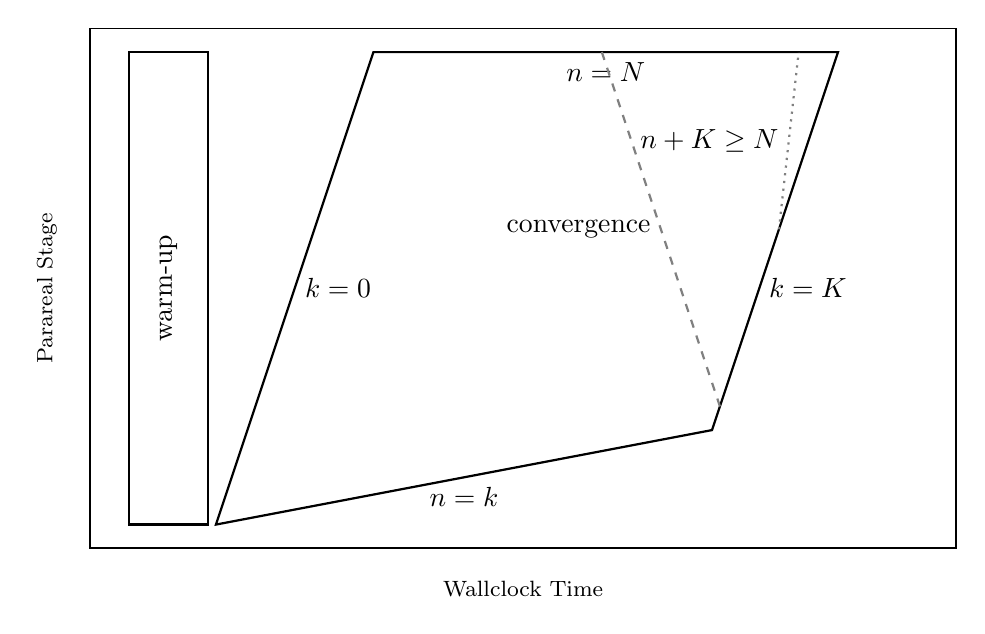
\begin{tikzpicture}
  \def\myscale{0.6}
  % axis and labels
  \node[below] at (5,-0.5*\myscale-0.3) {\footnotesize Wallclock Time};
  \node[rotate=90, above] at (-0.5-0.3,5*\myscale) {\footnotesize Parareal Stage};
\begin{scope}[yscale=\myscale]
  \draw[semithick] (-0.5,-0.5) rectangle (10.5,10.5);
  % timeline diagram
  \draw[thick] (0,0) rectangle node[rotate=90] {warm-up} (1,10);
  \draw[thick] (1.1,0)
    -- node[right] {$k=0$} (3.1,10)
    -- node[below] {$n=N$} (9,10)
    -- (7.4,2)
    -- node[below] {$n=k$} cycle;
  \node[right] at (8,5) {$k=K$};
  % lack of asynchronous data transfer
  \draw[thick,gray,dotted] (8.25,6.25)
    -- node[black,left] {$n+K \geq N$} (8.5,10);
  % early convergence due to "delta k = 1"
  \draw[thick,gray,dashed] (7.5,2.5)
    -- node[black,left] {convergence} (6,10);
\end{scope}
\end{tikzpicture}

  \caption[Revised schematic timeline diagram]{%
    Revised schematic timeline diagram of \julia{ParaReal.jl} implementation for $N$ stages and $K$ refinements.
    The dotted line is due to the lack of asynchronous data transfer for $n+k \geq N$,
    \cf~\autoref{sec:impl:pr:sync}.
    The dashed line indicates early convergence for $k_n < k_{n+1}$,
    \cf~\autoref{sec:impl:pr:conv}.
  }
  \label{fig:timeline:revised}
\end{figure}

\subsection{Advanced Scheduling Strategies}

\begin{itemize}
  \item
    Early stages $n=0,1,2$ become idle even before later stages receive their first $U^0_n$.
    Maybe they could be reused: measure runtime of $F$ and $G$ to compute optimum number $N$ for given number of processors.
    Alternatively, one could adjust the local time slices, \cf \url{https://gitlab.mpi-magdeburg.mpg.de/jschulze/ParaReal.jl/-/issues/2}
  \item
    If $X$ trajectories shall not be saved, solving the \ac{DRE} isn't that memory heavy.
    Creating a connection between workers in a cluster shouldn't be that expensive (they are initialized lazily, but cost should pay off).
    It might be worth it to send $U^{k+1}_n$ as well as $G(U^k_n)$ and $F(U^k_n)$ over the network in order to recycle processors.
    However, this requires a lazy DAG scheduling like \texttt{DAGGER.jl}.
  \item
    \cite[493]{Nielsen2018} relevant?
  \item
    Distributed processes vs local threads vs GPU?
\end{itemize}

\subsection{Parallel Programming Pitfalls}

\begin{itemize}
  \item
    \julia{@sync} may block\footnote{\url{https://github.com/JuliaLang/julia/issues/32677}}
    There is an experimental eager version,\footnote{\url{https://github.com/JuliaLang/julia/pull/34198}} but it doesn't support cancellation.
    In general, as of the time of writing this thesis,
    there is no recommended way to handle cancellation using the standard library,
    especially (and frustratingly) in a distributed environment.
  \item
    By default, unhandled concurrent errors are transient.\footnote{%
      \url{https://github.com/JuliaLang/julia/issues/10405}}
    That means that if a background task fails, not only does the program keep running, it doesn't even print an error.\footnote{%
      \url{https://github.com/JuliaLang/julia/pull/27722}}
    It is not easy to let unhandled concurrent errors crash the whole program.
    More severly, in a distributed environment, a failed task on one machine may easily cause a different machine to deadlock,
    \cf the previous paragraph.
    It is the user's (or the library developer's) responsibility to make errors observable,\footnote{%
      \url{https://github.com/JuliaLang/julia/pull/39518}}
    and to make sure that whole computation is properly cancelled.
  \item
    \url{https://github.com/JuliaLang/julia/issues/38931},
    \url{https://github.com/JuliaLang/julia/pull/44671}
\end{itemize}

\subsection{Where should I put this?}

\begin{itemize}
  \item
    Due to \autoref{thm:basics:dre-limit-are},
    I expect later parareal stages to require fewer Newton refinements to reach convergence.
    Therefore, each stage $n$ may defer the computation of a refinement $k$,
    until the previous stage $n-1$ finished computing its refinement $k+1$.
    That is, the number of refinements computed may differ by at most one from stage to stage.

    This effect is visible in the timeline diagram of \eg the reference solution of \autoref{fig:results:parareal:rail}.
\end{itemize}


\section{Numerical Results}

This section summarizes the results of applying the aforementioned methods to
the Rail benchmark~\cite{morwiki_steel} of size $n=371$
described in \eg~\autoref{thm:rail:parameters}.
Note that the algorithms are formulated for the problem stated in forwards time,
\begin{equation}
\left\{
\begin{aligned}
  E^\T \dot X E &= C^\T C + A^\T X E + E^\T X A - E^\T X BB^\T X E \\
  E^\T X(t_0) E &= \tfrac{1}{100} C^\T C
\end{aligned}
\right.
\end{equation}
but it's common practice to plot results in the time corresponding to the underlying \ac{OCP},
\ie $E^\T \tilde X(t_f) E = C^\T C/100$.

As described in \autoref{sec:HJT},
one is mainly interested in the accuracy of the feedback matrix
$
  K := B^\T X E \in \R^{7 \times n}
$.
For this purpose, the trajectory $K_{1,77}$ is characteristic due to its relatively large amplitude~\cite{Lang2015}.
Furthermore, the (global) relative error
\begin{equation}
\label{eq:results:err:ref}
  \frac{\norm{K(t) - K_\text{ref}(t)}_F}{\norm{K_\text{ref}(t)}_F}
\end{equation}
is analyzed \wrt a reference solution computed with the dense 4th order method described in \cite[Appendix~A]{Lang2017}.
Any error at $t=\SI{45}{\second}$ is not shown,
as it is zero due to the boundary condition of the \ac{DRE},
which would distort the overall diagram.

The tolerances for both the \ac{ADI} and parareal method,
\cf~\eqref{eq:adi:lrstop} in \autoref{sec:adi:lrstop}
and~\eqref{eq:impl:pr:conv} in \autoref{sec:impl:pr:conv},
are chosen to be $\epsilon := n\umach$
where $\umach$ denotes machine precision
and $n=371$ refers to the problem dimension.
The \ac{ADI} may perform up to 100 iterations.
A \ac{LRSIF} is compressed every 10 iterations or earlier,
if the inner dimension~$r$ reaches~$\onehalf n$,
\cf~\autoref{sec:impl:DRE}.
Furthermore, each of the $N = 450$ parareal stages requires two successive refinements without significant change
for (local) convergence,
while computing at most $K = 10$ refinements.

\begin{remark}
  In this subsection,
  $n$ may denote the problem dimension $X \in\Rnn$,
  or the time stop $t_n$,
  which is also related to the parareal stage $n$ corresponding to the time span $[t_{n-1}, t_n]$
  where $1 \leq n \leq N$.
  Furthermore,
  $K$ may denote the feedback matrix \mbox{$K = B^\T X E$},
  or the maximum number of parareal refinements $k_n \leq K$ computed per stage $n$.
  The particular meaning should be clear from its context.
\end{remark}

\subsection{Sequential Solvers}

\autoref{fig:results:sequential:rail} shows the results of the Rosenbrock schemes described in \autoref{sec:ros},
both in a dense and a \ac{LRSIF} formulation.
The low-rank variants are expected to perform identically to their dense counterparts,
which for \Ros{1} is ok.
However, there is a small difference between the second order methods for $t\leq\SI{44}{\second}$,
which destroys the order of \ac{LRSIF}~2 for about $t\leq\SI{35}{\second}$.
The general downward trend of the errors as $t$ approaches \SI{0}{\second} is due to the L-stability of the methods and the constant limit,
\cf~\autoref{thm:basics:dre-limit-are:backwards}.

\begin{figure}[tp]
  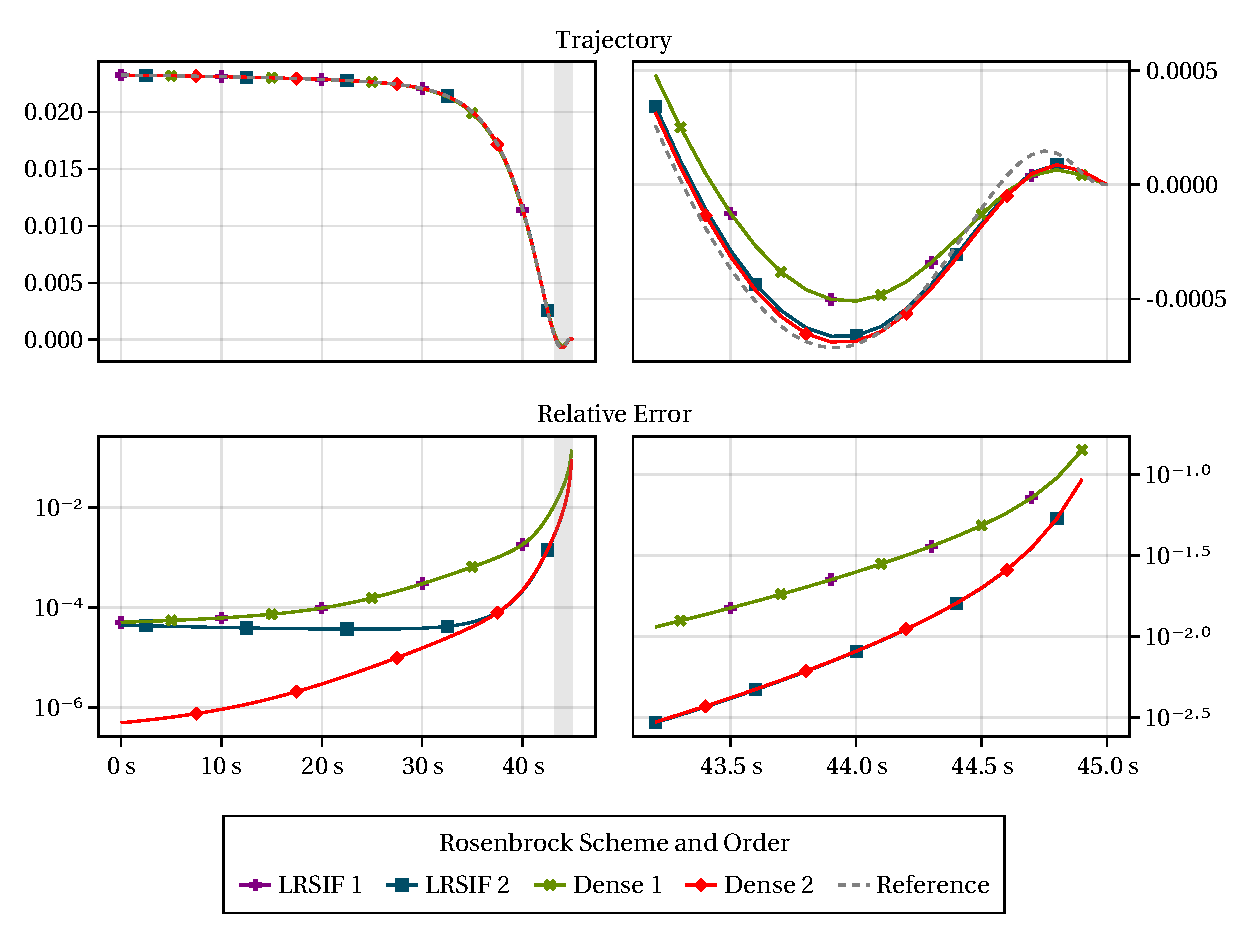
\includegraphics[width=\textwidth]{figures/fig_results_sequential.pdf}
  \caption[Rosenbrock method applied to Rail problem]{%
    Several Rosenbrock schemes applied to the problem of \autoref{thm:rail:parameters}.
    Each scheme performs 450 steps ($\tau = \SI{100}{\milli\second}$).
    Top: trajectory of $K_{1,77}$ (same as \cite[Fig.~1]{Lang2015}),
    % same as Lang2015, Fig. 1
    % Lang2017, Fig 6.1 used K_{1,71} instead
    bottom: relative error \eqref{eq:results:err:ref} compared to reference solution
    (900 steps of dense Rosenbrock scheme of order 4).
    Left: global time span $[\SI{0}{\second}, \SI{45}{\second}]$,
    right: zoom to $[\SI[round-mode=off]{43.2}{\second}, \SI{45}{\second}]$ (highlighted on the left).
  }
  \label{fig:results:sequential:rail}
\end{figure}

The problem of \ac{LRSIF}~2 can be confirmed with the (global) relative error
\begin{equation}
\label{eq:results:err:lr_v_dense}
  \frac{\norm{K_\text{\ac{LRSIF}}(t) - K_\text{Dense}(t)}_F}{\norm{K_\text{Dense}(t)}_F}
\end{equation}
between low-rank and dense variants of the same algorithm,
\cf~\autoref{fig:results:sequential:err}.
For \Ros{1} this value is within margin,
since $n \umach \approx 10^{-13}$.
However, for \Ros{2} there is a significant error from the very first iteration at $t=\SI[round-precision=1]{44.9}{\second}$.
This error stays about constant for the remainder of the time span.

\begin{figure}[tp]
  \centering
  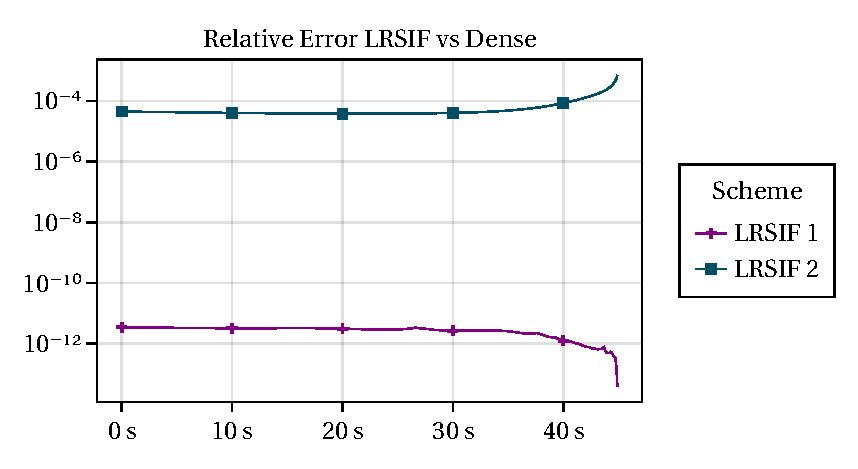
\includegraphics[width=0.75\textwidth]{figures/fig_results_sequential_err.pdf}
  \caption[Relative error between low-rank and dense solvers]{%
    Relative error \eqref{eq:results:err:lr_v_dense} in $K$ between low-rank and dense solvers
  }
  \label{fig:results:sequential:err}
\end{figure}

As mentioned in \autoref{thm:lowrank:rail},
the rank of $X$ should not get much larger than 113 along its trajectory.
\ac{LRSIF}~1 fulfills that expectation, as shown in \autoref{fig:results:sequential:rank}.
It grows quickly for $t > \SI{44}{\second}$ and seems to trend towards a plateau for $t< \SI{30}{\second}$.
\ac{LRSIF}~2, however, does not seem to stabilize,
which results in significantly larger ranks for about $t < \SI{40}{\second}$.

\begin{remark}
  \citeauthor{Lang2015}~\cite[63]{Lang2015} noted a problem with the low-rank version of \Ros{2} as well.
  The error behavior here looks similar to \cite[Fig~1]{Lang2015},
  keeping in mind that here the step size is $100\times$ larger
  and that the results are compared to dense solvers instead of \ac{LRCF} ones.
\end{remark}

\begin{figure}[tp]
  \centering
  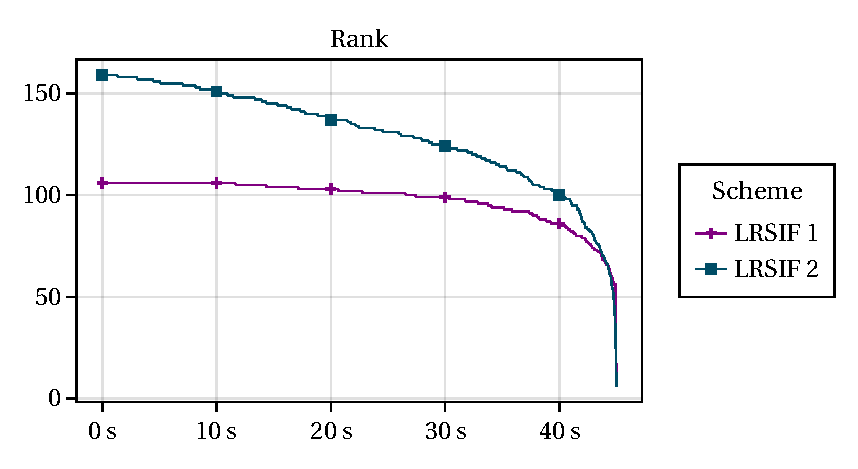
\includegraphics[width=0.7\textwidth]{figures/fig_results_sequential_rank.pdf}
  \caption[Numerical rank of low-rank sequential solutions to Rail problem]{%
    Numerical rank of low-rank sequential solutions $X$ to Rail problem,
    \cf~\cite[Figure~6.6b]{Lang2017}.
  }
  \label{fig:results:sequential:rank}
\end{figure}

The rank of the solution $X(t_n)$ has a major effect on the runtime of the next Rosenbrock step.
Recall that \Ros{1} leads to an \ac{ALE} whose right-hand is (a compression of) a \ac{LRSIF} of rank $q+r$
where $r := \rank X(t_n)$ denotes the rank of the previous Rosenbrock iterate.
Similarly, the right-hand side of the first stage of \Ros{2} is (a compression) of rank $q + 2r$.
The rank of the \ac{ADI} iterate thus grows by about that amount.
In the worst case, this causes a compression to be performed after every iteration of the \ac{ADI}.

\pagebreak

\subsection{Parareal Solvers}
\label{sec:results:parareal}

\autoref{fig:results:parareal:rail} shows the results of the parareal method described in \autoref{sec:pr}
for dense and \ac{LRSIF} algorithms and several order combinations.
Again, the schemes should perform identically for dense and \ac{LRSIF} storage.
As expected due to the problem discovered for \ac{LRSIF}~2,
this is true only for the parareal schemes of order 1/1 for their coarse/fine solver.
The reference solution has been computed with a dense order 4/4 parareal scheme.
Its $K_{1,77}$ trajectory is not shown as it would be indistinguishable from the other solutions.

\begin{figure}[tp]
  \centering
  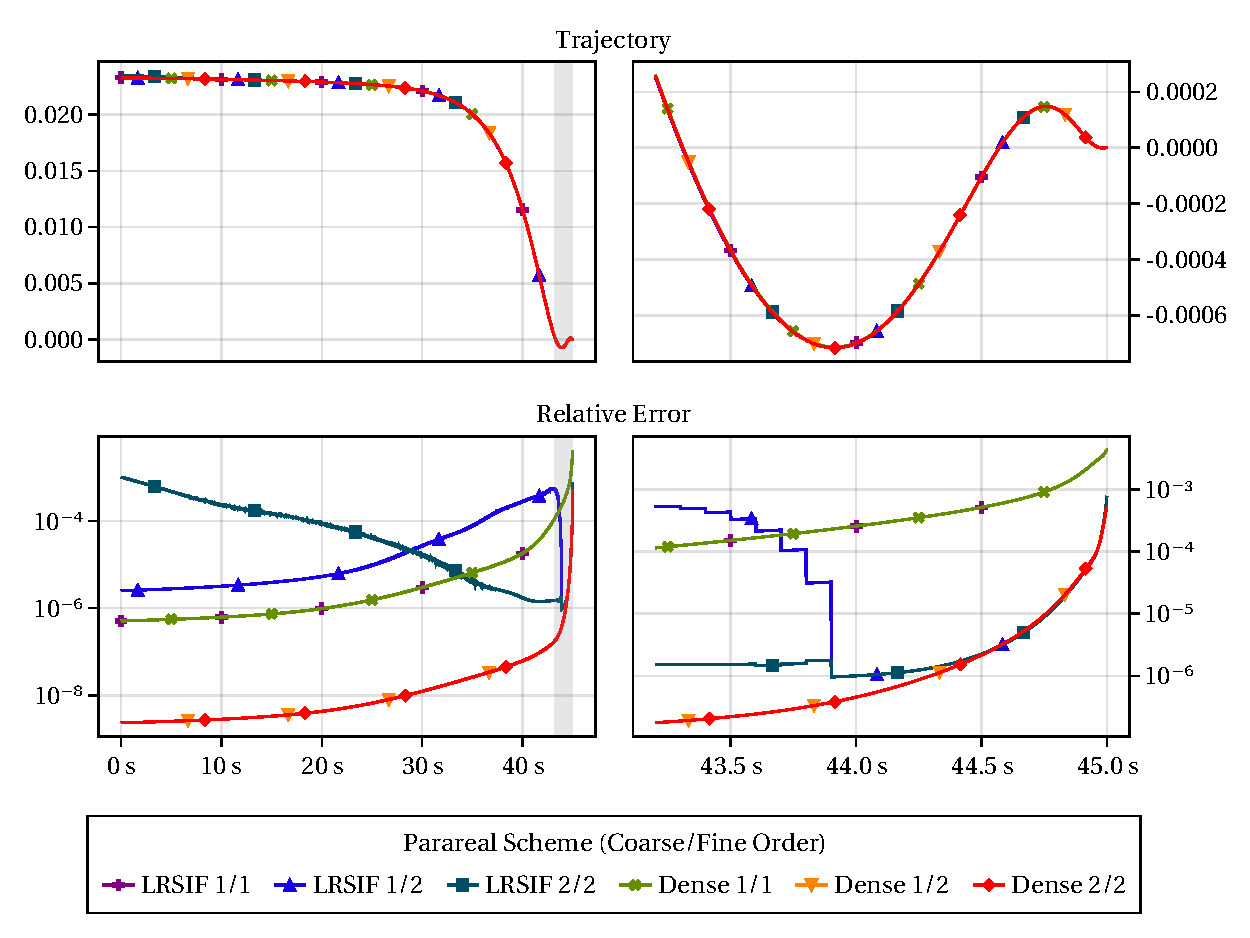
\includegraphics[width=\textwidth]{figures/fig_results_parareal.pdf}
  \caption[Parareal method applied to Rail problem]{%
    Several parareal schemes (Rosenbrock methods of given coarse/fine order)
    applied to the problem of \autoref{thm:rail:parameters},
    running on $N=450$ cores and
    computing up to $K=10$ refinements.
    Each scheme performs
    one coarse step ($\tau=\SI{100}{\milli\second}$) and
    100 fine steps ($\tau=\SI{1}{\milli\second}$) per stage.
    Top: trajectory of $K_{1,77}$ (same as \cite[Fig.~1]{Lang2015}),
    % same as Lang2015, Fig. 1
    % Lang2017, Fig 6.1 used K_{1,71} instead
    bottom: relative error \eqref{eq:results:err:ref} compared to reference solution
    (dense parareal scheme of order 4/4).
    Left: global time span $[\SI{0}{\second}, \SI{45}{\second}]$,
    right: zoom to $[\SI[round-mode=off]{43.2}{\second}, \SI{45}{\second}]$ (highlighted on the left).
  }
  \label{fig:results:parareal:rail}
\end{figure}

For the methods involving \ac{LRSIF}~2,
the relative error~\eqref{eq:results:err:ref} reveals
the typical discontinuities at the interval bounds
before convergence is reached,
\cf~\autoref{fig:pr:linear},
for $n > K = 10$ or $t \leq \SI[round-precision=1]{43.9}{\second}$.
But even for $t > \SI[round-precision=1]{43.9}{\second}$ the error of the low-rank variants is noticeably larger.
This effect has only been visible for $t < \SI{35}{\second}$ in the purely sequential setting,
\cf~\autoref{fig:results:sequential:rail}.
What looked like a more or less constant error in the previous subsection,
seems to be diverging in \autoref{fig:results:parareal:rail} for \ac{LRSIF}~2/2 as $t$ approaches $-\infty$,
which is in stark contrast to the otherwise downwards trend of the errors.
For about $t < \SI{28}{\second}$ the \ac{LRSIF}~2/2 solution is worse than the mixed order solution of \ac{LRSIF}~1/2.
Looking closely, the large error of \ac{LRSIF}~2/2 starts to become visible for $K_{1,77}$ around $t=\SI{0}{\second}$.


The rank of the solutions $X$ largely depends on the methods used,
\cf~\autoref{fig:results:parareal:rank}.
The parareal scheme \ac{LRSIF}~1/1 yields about the same ranks as the sequential \ac{LRSIF}~1.
Interestingly, the ranks of \ac{LRSIF}~1/2 are not much larger,
while showing the same plateau-effect.
This causes the runtimes $t_F(n, k_n)$ and $t_G(n, k_n)$ to not deviate too much for different $n$.
As can be seen in \autoref{fig:results:parareal:timeline},
all methods of order~1/1 and~1/2
reasonably fulfill the assumptions of the timeline model~\eqref{eq:impl:tpar} stated in \autoref{sec:impl:pr:warmup},
such that their timelines are close to the schematic in \autoref{fig:timeline:revised}.
This can be confirmed by the small error in $\hattpar$ in \autoref{tab:results:warmup}.
While for the dense methods this is to be expected,
it allows some observations to be made for the low-rank methods:
\begin{enumerate}
  \item
    \Ros{1} is barely affected by the larger rank,
    which causes \ac{LRSIF}~1/1 and \ac{LRSIF}~1/2 to have about the same ramp-up delay.
    This delay, however, is about \SI[round-precision=1]{0.2}{\second} larger than the overhead for the dense algorithms.
  \item
    Due to its two stages, \Ros{2} is more affected by the growing rank.
    Therefore, for \ac{LRSIF}~1/2 the runtime $t_F(n, k)$ is monotonic in $n$.
    Yet it is nearly constant in $k$,
    which causes the timeline diagram of \ac{LRSIF}~2/2
    to be narrow for early stages $n \leq 100$,
    and wider for later stages $n \geq 300$,
    without a noticeable gap between the refinements $k$.
\end{enumerate}
The second effect is visible for \ac{LRSIF}~1/1 as well, but not to that extent.

The rank of the solution $X$ obtained from the parareal scheme \ac{LRSIF}~2/2, however,
is even larger rank than the rank produced by the sequential \ac{LRSIF}~2,
while showing the same growth behavior (for decreasing $t$).
Neither of the methods of order 2/2 has a timeline diagram explained by~\eqref{eq:impl:tpar} or \autoref{fig:timeline:generic},
which is for the following reasons:
\begin{enumerate}[resume]
  \item
    Dense~2/2 does not fulfill the assumption that all stages $n$ compute the same number of refinements,
    \ie $k_n$ is not constant.
    Due to early convergence, \cf~\autoref{sec:impl:pr:conv},
    the last stage $n=N$ for example computes fewer refinements, $k_N = 7 < 10 = K$.
    This causes the runtime model~\eqref{eq:impl:tpar} to over-estimate the actual runtime,
    $\hattpar > \tpar$,
    as seen by the large error in \autoref{tab:results:warmup}.
  \item
    For \ac{LRSIF}~2/2 both runtimes $t_G(n, k)$ and $t_F(n, k)$ are monotonic in both $n$ (due to the growing rank) and $k$,
    while also having a big deviation from their median.
    The monotonicity in $k$ causes its timeline diagram to fan out,
    while the monotonicity in $n$ causes each \enquote{feathers} $k$ of the timeline diagram to be bent backwards.
    The resulting gaps between successive refinements $k$ on the final stage $n=N$ are not considered
    by the schematic timeline, \cf~\autoref{fig:timeline:revised}.
    Furthermore, the median over all $t_G(\optional{},\optional{})$ is much larger than,
    and therefore not a representative for $t_G(\optional{}, 0)$,
    which determines the slope of the $k=0$ face of the timeline.
    This causes the estimated ramp-up delay $\trampup$ to become negative.
    Both effects, the gaps on stage $n=N$ as well as $\trampup<0$,
    attribute to the runtime model~\eqref{eq:impl:tpar} under-estimating the actual runtime,
    $\hattpar < \tpar$,
    as seen by the large error in \autoref{tab:results:warmup}.
\end{enumerate}
The timeline diagram of the Dense~4/4 reference solution is shown in \autoref{fig:impl:restart},
which does not fulfill all the assumptions due to early convergence.

\begin{figure}[tp]
  \centering
  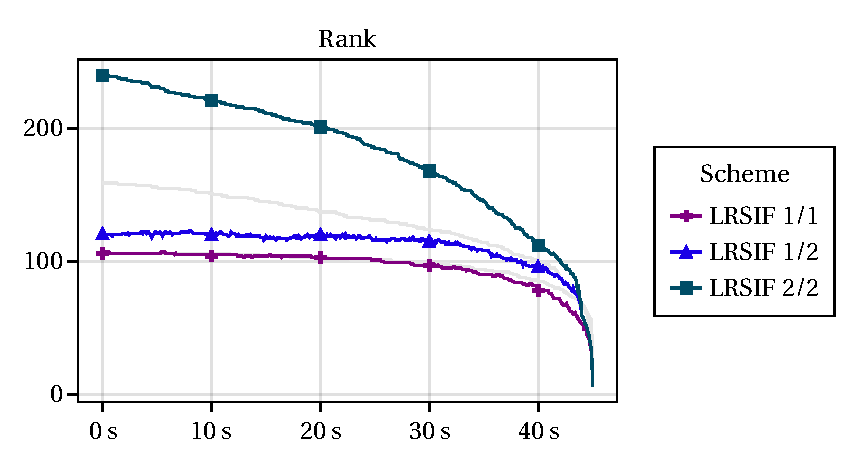
\includegraphics[width=0.7\textwidth]{figures/fig_results_parareal_rank.pdf}
  \caption[Numerical rank of low-rank parareal solutions to Rail problem]{%
    Numerical rank of low-rank parareal solutions to Rail problem,
    \cf~\cite[Figure~6.6b]{Lang2017}.
    Only values at parareal interfaces $t_n$ are shown,
    which coincide with the time steps of the sequential solutions.
    The numerical ranks of \autoref{fig:results:sequential:rail} are shown in the background.
  }
  \label{fig:results:parareal:rank}
\end{figure}

\begin{figure}[tp]
  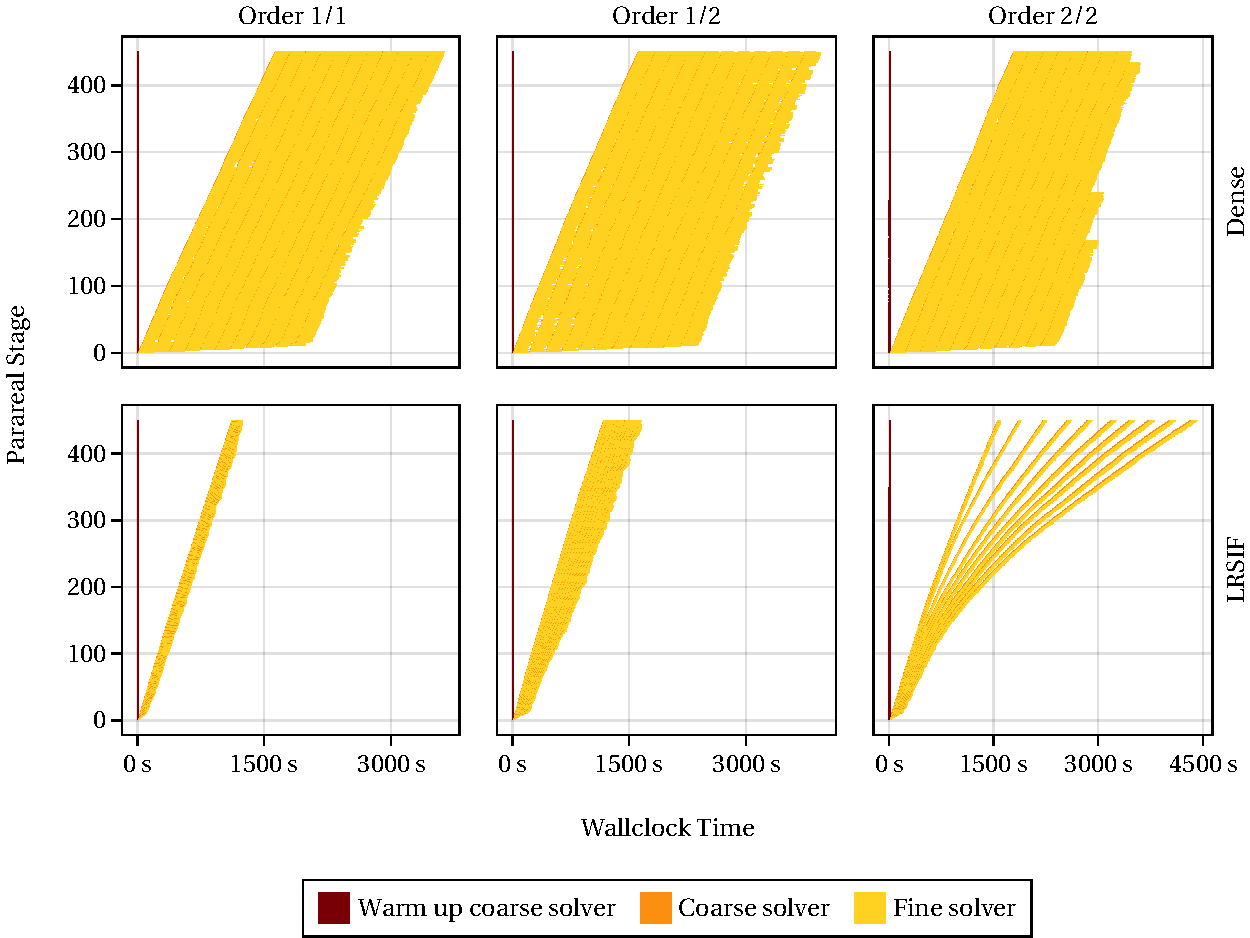
\includegraphics[width=\textwidth]{figures/fig_timeline_all.pdf}
  \caption[Timeline diagrams for parareal method applied to Rail problem]{%
    Timeline diagrams for the parareal methods applied to Rail problem.
    The schemes of coarse/fine order are as described in \autoref{fig:results:parareal:rail}.
  }
  \label{fig:results:parareal:timeline}
\end{figure}

\begin{table}[p]
  \centering
  \begin{tabular}{%
    l
    S[table-format=2] % k
    S[table-format=2.2] % warm-up
    S[table-format=-1.2] % ramp-up
    S[table-format=1.2] % G
    S[table-format=3.2] % F
    S[table-format=4.2] % par
    S[table-format=4.2] % par est
    S[round-precision=3, round-minimum=0.001, table-format=<1.3, scientific-notation=fixed, fixed-exponent=0] % err
  }
    \toprule
    Solver &
    {$k_N$} &
    {$\twarmup$} &
    {$\trampup$} &
    {$t_G$} &
    {$t_F$} &
    {$\tpar$} &
    {$\hattpar$} &
    {$\abs*{\frac{\hattpar-\tpar}{\tpar}}$} \\
    \midrule
    %TODO: Add uncertainties for low-rank t_F and t_G?
    LRSIF 1/1 & 10 & 18.126309871673584 & 1.9820044045989924 & 0.47998499870300293 & 9.849883079528809 & 1243.838875055313 & 1239.1701052194185 & 0.003753516576403047 \\
LRSIF 1/2 & 10 & 18.344510078430176 & 2.043351598200129 & 0.5375161170959473 & 32.58289909362793 & 1659.4842681884766 & 1543.5220331625312 & 0.06987847806025413 \\
LRSIF 2/2 & 10 & 21.727890968322754 & -1.6257711417956449 & 5.062106132507324 & 30.97498106956482 & 4417.833864927292 & 1959.4244898788647 & 0.5564739304855881 \\

    \addlinespace
    Dense 1/1 & 10 & 19.763540983200073 & 1.7398977895621996 & 1.8599169254302979 & 178.98965120315552 & 3627.2994508743286 & 3627.1654952188373 & 3.6929858509193245e-5 \\
Dense 1/2 & 10 & 19.545176029205322 & 1.7246065049500667 & 1.8416509628295898 & 209.07670402526855 & 3956.8617849349976 & 3942.621290436301 & 0.00359893654939238 \\
Dense 2/2 & 7 & 28.62309694290161 & 1.7665315399191162 & 2.167254090309143 & 209.65867733955383 & 3602.3622279167175 & 4126.744622183802 & 0.14556625932932343 \\

    \addlinespace
    Dense 4/4 & 4 & 28.806522130966187 & 1.6859412150818418 & 2.753262996673584 & 268.64974904060364 & 3381.8760890960693 & 5009.128286834284 & 0.48116848603201123 \\

    \bottomrule
  \end{tabular}
  \caption[Timeline measurements for parareal algorithm, $N=450$, $K=10$]{%
    Timeline measurements for parareal algorithm, $N=450$, $K=10$.
    All measurements and estimates are as in \autoref{tab:impl:warmup}.
    The first column denotes the parareal scheme (coarse/fine order).
    Refer to Figures \ref{fig:results:parareal:timeline} and \ref{fig:impl:restart} for the corresponding timelines.
  }
  \label{tab:results:warmup}
\end{table}

\begin{table}[p]
  \centering
  \begin{tabular}{%
    l
    S[table-format=4.2] % par
    S[table-format=6.2] % seq est
    S[table-format=2.2] % speedup
    S[round-precision=3, round-minimum=0.001, table-format=1.3, scientific-notation=fixed, fixed-exponent=0] % efficiency
  }
    \toprule
    Solver &
    {$\tpar$} &
    {$\hattseq$} &
    {$\frac{\hattseq}{\tpar}$} &
    {$\frac{\hattseq}{N\cdot\tpar}$} \\
    \midrule
    LRSIF 1/1 & 1243.838875055313 & 4313.1015791893005 & 3.4675725816959195 & 0.007705716848213155 \\
LRSIF 1/2 & 1659.4842681884766 & 14054.911208629608 & 8.469445283727943 & 0.018820989519395426 \\
LRSIF 2/2 & 4417.833864927292 & 24565.040289878845 & 5.560426453538251 & 0.012356503230085001 \\

    \addlinespace
    Dense 1/1 & 3627.2994508743286 & 75037.70862150192 & 20.686935180776086 & 0.0459709670683913 \\
Dense 1/2 & 3956.8617849349976 & 84595.60539913177 & 21.379469386879656 & 0.04750993197084368 \\
Dense 2/2 & 3602.3622279167175 & 89274.93912768364 & 24.78233266933632 & 0.05507185037630293 \\

    \addlinespace
    Dense 4/4 & 3381.8760890960693 & 115091.05863285065 & 34.03171955469633 & 0.07562604345488073 \\

    \bottomrule
  \end{tabular}
  \caption[Speed-up and parallel efficiency of parareal algorithm, $N=450$, $K=10$]{%
    Speed-up and parallel efficiency of parareal algorithm, $N=450$, $K=10$.
    This table complements \autoref{tab:results:warmup}.
    The sequential runtime $\hattseq$ is estimated according to~\eqref{eq:impl:tseq}.
    The parallel efficiency is evaluated for $N$ processors.
  }
  \label{tab:impl:pr:speedup}
\end{table}

\subsection{Runtime and Storage Size}

Refer to \autoref{tab:results:runtime} for the runtime and storage size of all resulting data sets.
Note that the ratios of the sizes of the data sets resulting from
sequential order~1 and parareal order~1/1
fit well to the estimated~1/3 of \autoref{thm:lowrank:rail}.
The other ratios are skewed by the rank problem of \ac{LRSIF}~\Ros{2}.

\begin{table}
  \centering
  \begin{tabular}{%
    lc
    % tau
    S[table-format=3]
    % runtime
    S[table-format=4]
    S[table-format=4]
    % size
    S[table-format=2.3, round-precision=3]
    S[table-format=2.3, round-precision=3]
  }
    \toprule
    &&&
    \multicolumn{2}{c}{Runtime [\si{\second}]} &
    \multicolumn{2}{c}{Size [\si{\gibi\byte}]} \\
    \cmidrule(rl){4-5}
    \cmidrule(rl){6-7}
    Solver & Order & {Resolution [\si{\milli\second}]} &
    {Dense} & {LRSIF} &
    {Dense} & {LRSIF} \\
    \midrule % jobid dense, lowrank
    Sequential & 1 & 100 & 217 & 599 & 0.472 & 0.165 \\ % 351941, 351939
    Sequential & 2 & 100 & 602 & 708 & 0.472 & 0.231 \\ % 351942, 351940
    \addlinespace
    Parareal & 1/1 & 1 & 4724 & 2366 & 47.047 & 15.971 \\ % 351236, 351158
    Parareal & 1/2 & 1 & 5057 & 2775 & 47.047 & 19.084 \\ % 351235, 351167
    Parareal & 2/2 & 1 & 4730 & 5519 & 47.047 & 35.161 \\ % 351290, 351160
    \addlinespace
    Sequential & 4 & 50 & 1785 & {--} & 0.942 & {--} \\ % 351965
    Parareal & 4/4 & 1 & 4512 & {--} & 47.047 & {--} \\ % 351270
    \bottomrule
  \end{tabular}
  \caption[Runtime and storage requirements]{%
    Overall runtime (as reported by Slurm)
    including time to write results to disk,
    and storage requirements of solutions to Rail benchmark~\cite{morwiki_steel}.
    The resolution is the step size $\tau$ of the (fine) solver.
    The storage size includes both $X$ and $K$ trajectories,
    storing only $K$ would result in substantially smaller files.
  }
  \label{tab:results:runtime}
\end{table}

